% This is samplepaper.tex, a sample chapter demonstrating the
% LLNCS macro package for Springer Computer Science proceedings;
% Version 2.21 of 2022/01/12
%
\documentclass[runningheads]{llncs}

\usepackage{color}
\usepackage[utf8]{inputenc}
\usepackage{fancyvrb}
\usepackage[usenames,dvipsnames]{xcolor}
\usepackage{listings}
\usepackage{booktabs}
\usepackage[most]{tcolorbox}

\lstdefinelanguage{Alloy}{
  keywords={all, and, as, assert, but, check, disj, else, exactly, extends, fact, for, fun, iden, if, iff, implies, in, Int, let, lone, module, no, none, not, one, open, or, pred, run, set, sig, some, sum, univ},
  keywordstyle=\color{blue}\bfseries,
  comment=[l][\color{Green}\bfseries]{//},
  morecomment=[s][\color{Green}]{/*}{*/},
  stringstyle=\color{red},
  morestring=[b]",
  sensitive=true
}

\lstset{
  language=Alloy,
  basicstyle=\ttfamily,
  numbers=none,
  showspaces=false,
  showstringspaces=false,
  showtabs=false,
  frame=none,
  tabsize=2,
  captionpos=b,
  breaklines=true,
  breakatwhitespace=false,
  escapeinside={\%*}{*)}
}


\lstdefinestyle{AlloyTable}{
  language=Alloy,
  basicstyle=\fontsize{8}{10}\ttfamily,
  numbers=none,
  backgroundcolor=\color{white},
  showspaces=false,
  showstringspaces=false,
  showtabs=false,
  frame=none,
  tabsize=2,
  breaklines=true,
  breakatwhitespace=false,
  aboveskip=0pt,
  belowskip=0pt
}

\tcbset{
    mytextbox/.style={
        colback=gray!10,
        colframe=white,
        boxrule=0pt,
        sharp corners,
        left=2mm,
        right=2mm,
        top=2mm,
        bottom=2mm,
    }
}

\fvset{commandchars=\\\{\}}

\newcommand{\BLUE}[1]{\textcolor{blue}{\textbf{#1}}}
\newcommand{\GREEN}[1]{\textcolor{Green}{\textbf{#1}}}
\newcommand{\RED}[1]{\textcolor{red}{\textbf{#1}}}

\usepackage{amssymb}
\usepackage{pifont}
\newcommand{\cmark}{\ding{51}}
\newcommand{\xmark}{\ding{55}}

\usepackage[T1]{fontenc}

\usepackage{graphicx}
% Used for displaying a sample figure. If possible, figure files should
% be included in EPS format.
%
% If you use the hyperref package, please uncomment the following two lines
% to display URLs in blue roman font according to Springer's eBook style:
%\usepackage{color}
%\renewcommand\UrlFont{\color{blue}\rmfamily}
%\urlstyle{rm}

%\usepackage{xcolor}
%\usepackage{fancyvrb}
%% \usepackage{xspace}
%% \usepackage{booktabs}
%% \usepackage{listings}
%% \usepackage{subfig}
%% \usepackage{url}
%% \usepackage{cite}
%% \usepackage{multirow}
%% \usepackage{wrapfig}
% \usepackage[sort&compress]{natbib}
\newcommand{\Comment}[1]{}
\newcommand{\CodeIn}[1]{\begin{small}\texttt{#1}\end{small}}
\newenvironment{CodeOut}{\vspace*{0ex}\begin{small}}
                        {\end{small}\vspace*{0ex}}

\newcommand{\Fix}[1]{\textcolor{red}{[#1]}}
\newcommand{\Intro}[1]{\emph{#1}}

\newcommand{\Blue}[1]{\textcolor{blue}{\textbf{#1}}}
\newcommand{\Green}[1]{\textcolor{Green}{\textbf{#1}}}
\newcommand{\Red}[1]{\textcolor{red}{\textbf{#1}}}

\newcommand{\ChatGPTUsed}{OpenAI o3-mini}
\newcommand{\DeepSeekUsed}{DeepSeek R1}
\newcommand{\NumSubjects}{11}
\newcommand{\NumTotalSynthesis}{22}
\newcommand{\NumTotalSketching}{11}
\newcommand{\NumTotalTasks}{33}


\begin{document}

\title{On the Effectiveness of Large Language Models in Writing Alloy
  Formulas}

\author{Yang Hong \and
Shan Jiang \and
Yulei Fu \and
Sarfraz Khurshid}

\authorrunning{Y. Hong, S. Jiang, Y. Fu, and S. Khurshid}

\institute{University of Texas at Austin, Austin TX 78712, USA
\email{\{yang22,shanjiang,yuleifu,khurshid\}@utexas.edu}}

\maketitle              % typeset the header of the contribution

\vspace*{-2ex}
\begin{abstract}  
Test time scaling is currently one of the most active research areas that shows promise after training time scaling has reached its limits.
Deep-thinking (DT) models are a class of recurrent models that can perform easy-to-hard generalization by assigning more compute to harder test samples.
However, due to their inability to determine the complexity of a test sample, DT models have to use a large amount of computation for both easy and hard test samples.
Excessive test time computation is wasteful and can cause the ``overthinking'' problem where more test time computation leads to worse results.
In this paper, we introduce a test time training method for determining the optimal amount of computation needed for each sample during test time.
We also propose Conv-LiGRU, a novel recurrent architecture for efficient and robust visual reasoning. 
Extensive experiments demonstrate that Conv-LiGRU is more stable than DT, effectively mitigates the ``overthinking'' phenomenon, and achieves superior accuracy.
\end{abstract}  
\section{Introduction}


\begin{figure}[t]
\centering
\includegraphics[width=0.6\columnwidth]{figures/evaluation_desiderata_V5.pdf}
\vspace{-0.5cm}
\caption{\systemName is a platform for conducting realistic evaluations of code LLMs, collecting human preferences of coding models with real users, real tasks, and in realistic environments, aimed at addressing the limitations of existing evaluations.
}
\label{fig:motivation}
\end{figure}

\begin{figure*}[t]
\centering
\includegraphics[width=\textwidth]{figures/system_design_v2.png}
\caption{We introduce \systemName, a VSCode extension to collect human preferences of code directly in a developer's IDE. \systemName enables developers to use code completions from various models. The system comprises a) the interface in the user's IDE which presents paired completions to users (left), b) a sampling strategy that picks model pairs to reduce latency (right, top), and c) a prompting scheme that allows diverse LLMs to perform code completions with high fidelity.
Users can select between the top completion (green box) using \texttt{tab} or the bottom completion (blue box) using \texttt{shift+tab}.}
\label{fig:overview}
\end{figure*}

As model capabilities improve, large language models (LLMs) are increasingly integrated into user environments and workflows.
For example, software developers code with AI in integrated developer environments (IDEs)~\citep{peng2023impact}, doctors rely on notes generated through ambient listening~\citep{oberst2024science}, and lawyers consider case evidence identified by electronic discovery systems~\citep{yang2024beyond}.
Increasing deployment of models in productivity tools demands evaluation that more closely reflects real-world circumstances~\citep{hutchinson2022evaluation, saxon2024benchmarks, kapoor2024ai}.
While newer benchmarks and live platforms incorporate human feedback to capture real-world usage, they almost exclusively focus on evaluating LLMs in chat conversations~\citep{zheng2023judging,dubois2023alpacafarm,chiang2024chatbot, kirk2024the}.
Model evaluation must move beyond chat-based interactions and into specialized user environments.



 

In this work, we focus on evaluating LLM-based coding assistants. 
Despite the popularity of these tools---millions of developers use Github Copilot~\citep{Copilot}---existing
evaluations of the coding capabilities of new models exhibit multiple limitations (Figure~\ref{fig:motivation}, bottom).
Traditional ML benchmarks evaluate LLM capabilities by measuring how well a model can complete static, interview-style coding tasks~\citep{chen2021evaluating,austin2021program,jain2024livecodebench, white2024livebench} and lack \emph{real users}. 
User studies recruit real users to evaluate the effectiveness of LLMs as coding assistants, but are often limited to simple programming tasks as opposed to \emph{real tasks}~\citep{vaithilingam2022expectation,ross2023programmer, mozannar2024realhumaneval}.
Recent efforts to collect human feedback such as Chatbot Arena~\citep{chiang2024chatbot} are still removed from a \emph{realistic environment}, resulting in users and data that deviate from typical software development processes.
We introduce \systemName to address these limitations (Figure~\ref{fig:motivation}, top), and we describe our three main contributions below.


\textbf{We deploy \systemName in-the-wild to collect human preferences on code.} 
\systemName is a Visual Studio Code extension, collecting preferences directly in a developer's IDE within their actual workflow (Figure~\ref{fig:overview}).
\systemName provides developers with code completions, akin to the type of support provided by Github Copilot~\citep{Copilot}. 
Over the past 3 months, \systemName has served over~\completions suggestions from 10 state-of-the-art LLMs, 
gathering \sampleCount~votes from \userCount~users.
To collect user preferences,
\systemName presents a novel interface that shows users paired code completions from two different LLMs, which are determined based on a sampling strategy that aims to 
mitigate latency while preserving coverage across model comparisons.
Additionally, we devise a prompting scheme that allows a diverse set of models to perform code completions with high fidelity.
See Section~\ref{sec:system} and Section~\ref{sec:deployment} for details about system design and deployment respectively.



\textbf{We construct a leaderboard of user preferences and find notable differences from existing static benchmarks and human preference leaderboards.}
In general, we observe that smaller models seem to overperform in static benchmarks compared to our leaderboard, while performance among larger models is mixed (Section~\ref{sec:leaderboard_calculation}).
We attribute these differences to the fact that \systemName is exposed to users and tasks that differ drastically from code evaluations in the past. 
Our data spans 103 programming languages and 24 natural languages as well as a variety of real-world applications and code structures, while static benchmarks tend to focus on a specific programming and natural language and task (e.g. coding competition problems).
Additionally, while all of \systemName interactions contain code contexts and the majority involve infilling tasks, a much smaller fraction of Chatbot Arena's coding tasks contain code context, with infilling tasks appearing even more rarely. 
We analyze our data in depth in Section~\ref{subsec:comparison}.



\textbf{We derive new insights into user preferences of code by analyzing \systemName's diverse and distinct data distribution.}
We compare user preferences across different stratifications of input data (e.g., common versus rare languages) and observe which affect observed preferences most (Section~\ref{sec:analysis}).
For example, while user preferences stay relatively consistent across various programming languages, they differ drastically between different task categories (e.g. frontend/backend versus algorithm design).
We also observe variations in user preference due to different features related to code structure 
(e.g., context length and completion patterns).
We open-source \systemName and release a curated subset of code contexts.
Altogether, our results highlight the necessity of model evaluation in realistic and domain-specific settings.





% !TEX root = main.tex

\begin{figure}[t]
\vspace{-1.5cm}
\begin{minipage}{0.34\textwidth}
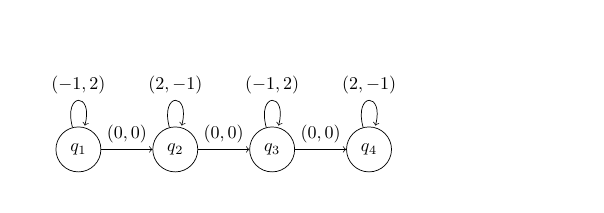
\begin{tikzpicture}[scale=0.25]
\usetikzlibrary{automata, positioning}
\scalebox{0.65}{
\node[state] (q1) {$q_1$};
\node[state, right=of q1] (q2) {$q_2$};
\node[state, right=of q2] (q3) {$q_3$};
\node[state, right=of q3] (q4) {$q_4$};

\path[->] (q1) edge [loop above] node[above] {$(-1,2)$} (q1) edge node[above] {$(0,0)$} (q2); 
\path[->] (q2) edge [loop above] node[above] {$(2,-1)$} (q2) edge node[above] {$(0,0)$} (q3);
\path[->] (q3) edge [loop above] node[above] {$(-1,2)$} (q3) edge node[above] {$(0,0)$} (q4);
\path[->] (q4) edge [loop above] node[above] {$(2,-1)$} (q4);
}
\end{tikzpicture}
\end{minipage}
\begin{minipage}{0.32\textwidth}
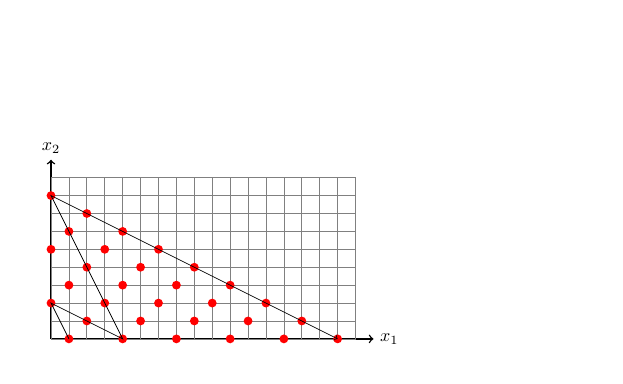
\begin{tikzpicture}[scale=0.35]
\scalebox{0.65}{
\draw[->, thick] (0, 0) -- (18, 0) node[right] {$x_1$};
\draw[->, thick] (0, 0) -- (0, 10) node[above] {$x_2$};

\draw[step=1, gray, thin] (0, 0) grid (17, 9);

\foreach \x in {1,4,7,10,13,16} \fill[red] (\x,0) circle (7pt);
\foreach \x in {2,5,8,11,14} \fill[red] (\x,1) circle (7pt);
\foreach \x in {0,3,6,9,12} \fill[red] (\x,2) circle (7pt);
\foreach \x in {1,4,7,10} \fill[red] (\x,3) circle (7pt);
\foreach \x in {2,5,8} \fill[red] (\x,4) circle (7pt);
\foreach \x in {0,3,6} \fill[red] (\x,5) circle (7pt);
\foreach \x in {1,4} \fill[red] (\x,6) circle (7pt);
\foreach \x in {2} \fill[red] (\x,7) circle (7pt);
\foreach \x in {0} \fill[red] (\x,8) circle (7pt);

\draw[->] (1,0) -- (0,2) -- (2,1) -- (4,0) -- (3,2) -- (2,4) -- (1,6) -- (0,8) -- (2,7) -- (4,6) -- (6,5) -- (8,4) -- (10,3) -- (12,2) -- (14,1) -- (16,0);
}
\end{tikzpicture}
\end{minipage}
\begin{minipage}{0.32\textwidth}
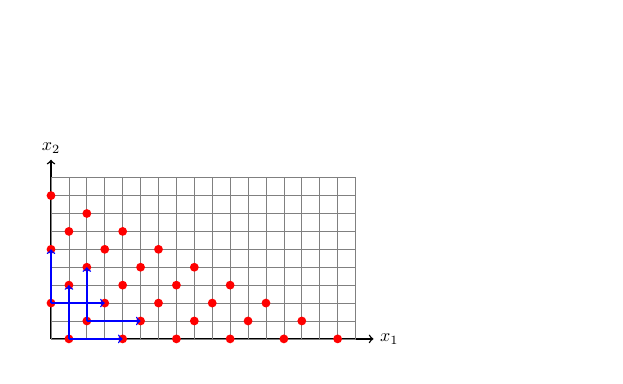
\begin{tikzpicture}[scale=0.35]
\scalebox{0.65}{
\draw[->, thick] (0, 0) -- (18, 0) node[right] {$x_1$};
\draw[->, thick] (0, 0) -- (0, 10) node[above] {$x_2$};

\draw[step=1, gray, thin] (0, 0) grid (17, 9);

\foreach \x in {1,4,7,10,13,16} \fill[red] (\x,0) circle (7pt);
\foreach \x in {2,5,8,11,14} \fill[red] (\x,1) circle (7pt);
\foreach \x in {0,3,6,9,12} \fill[red] (\x,2) circle (7pt);
\foreach \x in {1,4,7,10} \fill[red] (\x,3) circle (7pt);
\foreach \x in {2,5,8} \fill[red] (\x,4) circle (7pt);
\foreach \x in {0,3,6} \fill[red] (\x,5) circle (7pt);
\foreach \x in {1,4} \fill[red] (\x,6) circle (7pt);
\foreach \x in {2} \fill[red] (\x,7) circle (7pt);
\foreach \x in {0} \fill[red] (\x,8) circle (7pt);

\draw[->,blue,thick] (1,0) -- (4,0);
\draw[->,blue,thick] (1,0) -- (1,3);

\draw[->,blue,thick] (2,1) -- (5,1);
\draw[->,blue,thick] (2,1) -- (2,4);

\draw[->,blue,thick] (0,2) -- (3,2);
\draw[->,blue,thick] (0,2) -- (0,5);
}
\end{tikzpicture}
\end{minipage}
\caption{Left: 4-component \dvass $V_2$. 
Middle: the set $\reach_{q_4}(V_2, q_1(1,0))$ and a path $q_1(1,0) \tran q_4(16,0)$.
Right: bases 
%$A = \{(1,0),(2,1),(0,2)\}$ 
and periods 
%$P = \{(0,3),(3,0)\}$
 of an over-approximating semi-linear set $A+P^*$.}
\label{fig:zigzag}
\end{figure}

\begin{example}
For $k\geq 1$, let $V_k$ be a $(2k)$-component \dvass, where each component has just one state $q_i$
and one transition:
$(q_i, (-1,2), q_i)$ for odd $i$, and $(q_i, (2,-1), q_i)$ for even $i$.
Bridge transitions are $(q_i, (0,0), q_{i+1})$.
Figure~\ref{fig:zigzag} shows $V_2$ (left) and 
a path in $V_2$ from $s = q_1(1,0)$ to $t = q_4(16,0)$ together with 
the reachability set $\reach_{q_4}(V_2, s)$ (middle).
In general,
\begin{align} \label{eq:reachk}
X_k := \reach_{q_{2k}}(V_k, s) \ = \ \set{(x_1,x_2) \mid x_1+2x_2 \leq 4^k, \  x_1+2x_2 \equiv 1 \!\! \mod 3}.
\end{align}
Even if the size of the reachability set is 
exponential in $k$, for small $(x_1, x_2)$ it is periodic and the periods are small.
The set $X_k$ can be over-approximated by $A + P^*$ for $A = \set{(1,0),(2,1),(0,2)}$ and $P = \set{(0,3),(3,0)}$
(shown on the right of Figure~\ref{fig:zigzag}), namely for every $k\geq 1$ and $B\in\N$,
the set $X_k$ is \kanapka {$8$} {$B$}. 
For illustration, consider $Y := X_k \cap ((1,0) + P^*)$.
If $(1,0) + P^{\leq B} \subseteq X_k$ then $Y$ is a $B$-approximation
of $(1,0) + P^*$ with $\norm((1,0)), \norm(P) \leq 3 \leq 8$. 
Otherwise, there is some $(v_1, v_2) \in \big((1,0) + P^{\leq B}\big)\setminus X_k$, and
then $B$ is larger than $4^k$:
\[
%8B \geq 2(1 + 3B) \geq 2(v_1 + v_2) \geq v_1 + 2 v_2 > 
4^k < v_1 + 2 v_2 \leq 2(v_1 + v_2) \leq 2(1+3B) \leq 8B.
\]
Therefore by \eqref{eq:reachk}, each $(x_1,x_2) \in Y$ satisfies 
$\norm(x_1,x_2) = x_1 + x_2 \leq x_1 + 2x_2 \leq 4^k < 8B$, and thus
$Y$, seen as a union of singletons, is a union of 
linear sets with norm of base bounded by $8B$ and empty set of periods. 
In both cases, 
$Y$ is \kanapka {$8$} {$B$}. 
%The same intuition stays behind polynomial approximability of \dvass stated in Lemma~\ref{lem:2vass-sandwich}.
\end{example}
\section{Temporal Representation Alignment}
\label{sec:approach}

When training a series of short-horizon goal-reaching and instruction-following tasks, our goal is to learn a representation space such that our policy can generalize to a new (long-horizon) task that can be viewed as a sequence of known subtasks.
We propose to structure this representation space by aligning the representations of states, goals, and language in a way that is more amenable to compositional generalization.

\paragraph{Notation.}
We take the setting of a goal- and language-conditioned MDP $\cM$ with state space $\cS$, continuous action space $\cA \subseteq (0,1)^{d_{\cA}}$, initial state distribution $p_0$, dynamics $\p(s'\mid s,a)$, discount factor $\gamma$, and language task distribution $p_{\ell}$.
A policy $\pi(a\mid s)$ maps states to a distribution over actions. We inductively define the $k$-step (action-conditioned) policy visitation distribution as:
\begin{align*}
    p^{\pi}_{1}(s_{1} \mid s_1, a_{1})
    &\triangleq p(s_1 \mid s_1, a_1),\\
    p^{\pi}_{k+1}(s_{k+1} \mid s_1, a_1)
    &\triangleq \nonumber\\*
      &\mspace{-120mu} \int_{\cA}\int_{\cS} p(s_{k+1} \mid s,a) \dd p^{\pi}_{k}(s \mid s_{1},a_1) \dd
        \pi(a \mid s)\\
    p^{\pi}_{k+t}(s_{k+t} \mid s_t,a_t)
    &\triangleq p^{\pi}(s_{k} \mid s_1, a_1) . \eqmark
        \label{eq:successor_distribution}
\end{align*}
Then, the discounted state visitation distribution can be defined as the distribution over $s^{+}$\llap, the state reached after $K\sim \operatorname{Geom}(1-\gamma)$ steps:
\begin{equation}
    p^{\pi}_{\gamma}(s^{+}  \mid  s,a) \triangleq \sum_{k=0}^{\infty} \gamma^{k} p^{\pi}_{k}(s^{+} \mid s,a).
    \label{eq:discounted_state_visitation}
\end{equation}

We assume access to a dataset of expert demonstrations $\cD = \{\tau_{i},\ell_i\}_{i=1}^{K}$, where each trajectory
\begin{equation}
    \tau_{i} = \{s_{t,i},a_{t,i}\}_{t=1}^{H} \in \cS \times \cA
    \label{eq:trajectory}
\end{equation}
is gathered by an expert policy $\expert$, and is then annotated with $p_{\ell}(\ell_{i} \mid s_{1,i}, s_{H,i})$.
Our aim is to learn a policy $\pi$ that can select actions conditioned on a new language instruction $\ell$.
As in prior work~\citep{walke2023bridgedata}, we handle the continuous action space by representing both our policy and the expert policy as an isotropic Gaussian with fixed variance; we will equivalently write $\pi(a\mid s, \varphi)$ or denote the mode as $\hat{a} = \pi(s,\varphi)$ for a task $\varphi$.

\begin{rebuttal}
    \subsection{Representations for Reaching Distant Goals}
    \label{sec:reaching_goals}

    We learn a goal-conditioned policy $\pi(a\mid s,g)$ that selects actions to reach a goal $g$ from expert demonstrations with behavioral cloning.
    Suppose we directly selected actions to imitate the expert on two trajectories in $\cD$:
    
    \begin{equation}
        \mspace{-100mu}\begin{tikzcd}[remember picture,sep=small]
            s_1 \rar & s_2 \rar  & \ldots \rar & s_{H} \rar & w      \quad \\
            w \rar   & s_1' \rar & \ldots \rar & s_{H}' \rar & g\quad
        \end{tikzcd}
        \begin{tikzpicture}[remember picture,overlay] \coordinate (a) at (\tikzcdmatrixname-1-5.north east);
            \coordinate (b) at (\tikzcdmatrixname-2-5.south east);
            \coordinate (c) at (a|-b);
            \draw[decorate,line width=1.5pt,decoration={brace,raise=3pt,amplitude=5pt}]
        (a) -- node[right=1.5em] {$\tau_{i}\in \cD$} (c); \end{tikzpicture}
        \label{eq:trajectory_diagram}
    \end{equation}
    When conditioned with the composed goal $g$, we would be unable to imitate effectively
        as the composed state-goal $(s,g)$ is jointly out of the training distribution.

    What \emph{would} work for reaching $g$ is to first condition the policy on the intermediate waypoint $w$, then upon reaching $w$, condition on the goal $g$, as the state-goal pairs $(s_{i},w)$, $(w,g)$, and $(s_{i}',g)$ are all in the training distribution.
    If we condition the policy on some intermediate waypoint distribution $p(w)$ (or sufficient statistics thereof) that captures all of these cases, we can stitch together the expert behaviors to reach the goal $g$.

    Our approach is to learn a representation space that captures this ability, so that a GCBC objective used in this space can effectively imitate the expert on the composed task.
     We begin with the goal-conditioned behavioral cloning~\citep{kaelbling1993learning}
        loss $\cL_{\textsc{bc}}^{\phi,\psi,\xi}$ conditioned with waypoints $w$.
    \begin{equation}
        \cL_{\textsc{bc}}\bigl(\{s_{i},a_{i},s_{i}^{+},g_{i}\}_{i=1}^{K}\bigr) = \sum_{{i=1}}^{K} \log \pi\bigl(a_{i} \mid s_{i},\psi(g_{i})\bigr).
        \label{eq:goal_conditioned_bc}
    \end{equation}
    Enforcing the invariance needed to stitch \cref{eq:trajectory_diagram} then reduces to aligning \mbox{$\psi(g) \leftrightarrow \psi(w).$}
    The temporal alignment objective $\phi(s)\leftrightarrow \phi(s^{+})$ accomplishes this indirectly by aligning both $\psi(w)$ and $\psi(g)$ to the shared waypoint representation $\phi(w)$:

    \csuse{color indices}
    \begin{align}
        &\cL_{\textsc{nce}}\bigl(\{s_{i},s_{i}^{+}\}_{i=1}^{K};\phi,\psi\bigr) =
        \log \biggl( {\frac{e^{\phi(s^+_{\i})^{T}\psi(s_{\i})}}{\sum_{{\j=1}}^{K}
                e^{\phi(s^+_{\i})^{T}\psi(s_{\j})}}} \biggr)  \nonumber\\*
                &\mspace{100mu} +
        \sum_{{\j=1}}^{K} \log \biggl( {\frac{e^{\phi(s^+_{\i})^{T}\psi(s_{\i})}}{\sum_{{\i=1}}^{K}
                e^{\phi(s^+_{\i})^{T}\psi(s_{\j})}}} \biggr)
        \label{eq:goal_alignment}
    \end{align}

        
\end{rebuttal}
\subsection{Interfacing with Language Instructions}
\label{sec:language_instructions}

To extend the representations from \cref{sec:reaching_goals} to compositional instruction following with language tasks, we need some way to ground language into the $\psi$ (future state)
representation space.
We use a similar approach to GRIF~\citep{myers2023goal}, which uses an additional CLIP-style \citep{radford2021learning} contrastive alignment loss with an additional pretrained language encoder $\xi$:
\csuse{no color indices}
\begin{align}
    &\cL_{\textsc{nce}}\bigl(\{g_{i},\ell_{i}\}_{i=1}^{K};\psi,\xi\bigr)
    = \sum_{{i=1}}^{K} \log \biggl( {\frac{e^{\psi(g_{\i})^{T}\xi(\ell_{\i})}}{\sum_{{\j=1}}^{K}
            e^{\psi(g_{\i})^{T}\xi(\ell_{\j})}}} \biggr)  \nonumber\\*
            &\mspace{100mu} +
    \sum_{{\j=1}}^{K} \log \biggl( {\frac{e^{\psi(g_{\i})^{T}\xi(\ell_{\i})}}{\sum_{{\i=1}}^{K}
            e^{\psi(g_{\i})^{T}\xi(\ell_{\j})}}} \biggr)
    \label{eq:task_alignment}
\end{align}

\subsection{Temporal Alignment}
\label{sec:temporal_alignment}

Putting together the objectives from \cref{sec:reaching_goals,sec:language_instructions} yields the Temporal Representation Alignment (\Method) approach.
\Method{} structures the representation space of goals and language instructions to better enable compositional generalization.
We learn encoders $\phi, \psi ,$ and $\xi$ to map states, goals, and language instructions to a shared representation space.

\csuse{color indices}
\begin{align}
    \cL_{\textsc{nce}} \label{eq:NCE}
    &(\{x_{i}, y_{i}\}_{i=1}^{K};f,h) =
        \sum_{{\i=1}}^{K} \log \biggl( {\frac{e^{f(y_{\i})^{T}h(x_{\i})}}{\sum_{{\j=1}}^{K}
        e^{f(y_{\i})^{T}h(x_{\j})}}} \biggr) \nonumber\\*
      &\mspace{100mu} +
        \sum_{{\j=1}}^{K} \log \biggl( {\frac{e^{f(y_{\i})^{T}h(x_{\i})}}{\sum_{{\i=1}}^{K}
        e^{f(y_{\i})^{T}h(x_{\j})}}} \biggr) \\
    \cL_{\textsc{bc}} \label{eq:BC}
    &\bigl(\{s_{i},a_{i},s^{+}_{i},\ell_{i}\}_{i=1}^{K};\pi,\psi,\xi\bigr) = \nonumber\\*
      &\mspace{-10mu} \sum_{{i=1}}^{K} \log
        \pi\bigl(a_{i} \mid s_{i},\xi(\ell_{i})\bigr) + \log \pi\bigl(a_{i} \mid
        s_{i},\psi(s^{+}_{i})\bigr) \\
    \cL_{\textsc{tra}}
    &\label{eq:TRA} \bigl( \{s_{i},a_{i},s_{i}^{+},g_{i},\ell_{i}\}_{i=1}^{K}; \pi,\phi,\psi,\xi\bigr)
        \\
    &= \underbrace{\cL_{\textsc{bc}}\bigl(\{s_{i},a_{i},s_{i}^{+},\ell_{i}\}_{i=1}^{K};\pi,\psi,\xi\bigr)}_{\text{behavioral
    cloning}} \nonumber\\*
    &+
        \underbrace{\cL_{\textsc{nce}}\bigl(\{s_{i},s_{i}^{+}\}_{i=1}^{K};\phi,\psi\bigr)}_{\text{temporal alignment}}
        + \underbrace{\cL_{\textsc{nce}}\bigl(\{g_{i},\ell_{i}\}_{i=1}^{K};\psi,\xi\bigr)}_{\text{task alignment}} \nonumber
\end{align}Note that the NCE alignment loss uses a CLIP-style symmetric contrastive objective~\citep{radford2021learning,eysenbach2024inference} \-- we highlight the indices in the NCE alignment loss~\eqref{eq:NCE} for clarity.

Our overall objective is to minimize \cref{eq:TRA} across states, actions, future states, goals, and language tasks within the training data:
\begin{align}
    &\min_{\pi,\phi,\psi,\xi} \mathbb{E}_{\substack{(s_{1,i},a_{1,i},\ldots,s_{H,i},a_{H,i},\ell) \sim \mathcal{D} \\
    i\sim\operatorname{Unif}(1\ldots H) \\
    k\sim\operatorname{Geom}(1-\gamma)}} \\*
    &\mspace{10mu}
    \Bigl[\cL_{\text{TRA}}\bigl(\{s_{t,i},a_{t,i},s_{\min(t+k,H),i},s_{H,i},\ell\}_{i=1}^{K};\pi,\phi,\psi,\xi\bigr)\Bigr].
    \label{eq:overall_objective}
\end{align}

\begin{algorithm}
    \caption{Temporal Representation Alignment}
    \label{alg:tra}
    \begin{algorithmic}[1]
        \State \textbf{input:} dataset $\mathcal{D} = (\{s_{t,i},a_{t,i}\}_{t=1}^{H},\ell_i)_{i=1}^N$
        \State initialize networks $\Theta \triangleq (\pi,\phi,\psi,\xi)$
        \While{training}
        \State sample batch $\bigl\{(s_{t,i},a_{t,i},s_{t+k,i},\ell_i)\bigr\}_{i=1}^K\sim\mathcal{D}$ \\
        \hspace*{2ex} for $k\sim\operatorname{Geom}(1-\gamma)$
        \State $\Theta \gets \Theta - \alpha \nabla_{\Theta} \cL_{\text{TRA}}\bigl(\{s_{t,i},a_{t,i},s_{t+k,i},\ell_i\}_{i=1}^K; \Theta\bigr)$
        \EndWhile
        \smallskip
        \State \textbf{output:} \parbox[t]{\linewidth}{language-conditioned policy $\pi(a_{t} | s_{t}, \xi(\ell))$ \\
            goal-conditioned policy $\pi(a_{t} | s_{t}, \psi(g))$
        }
    \end{algorithmic}
\end{algorithm}

\subsection{Implementation}
\label{sec:implementation}

A summary of our approach is shown in \cref{alg:tra}.
In essence, TRA learns three encoders: $\phi$, which encodes states, $\psi$ which encodes future goals, and $\xi$ which encodes language instructions.
Contrastive losses are used to align state representations $\phi(s_{t})$ with future goal representations $\psi(s_{t+k})$, which are in turn aligned with equivalent language task specifications $\xi(\ell)$ when available.
We then learn a behavior cloning policy $\pi$ that can be conditioned on either the goal or language instruction through the representation $\psi(g)$ or $\xi(\ell)$, respectively.

\begin{rebuttal}
    \subsection{Temporal Alignment and Compositionality}
    \label{sec:compositionality}

    We will formalize the intuition from \cref{sec:reaching_goals} that \Method{} enables compositional generalization by considering the error on a ``compositional'' version of $\cD,$ denoted $\cD^{*}$.
    Using the notation from \cref{eq:trajectory}, we can say $\cD$ is distributed according to:
    \begin{align}
        &\cD \triangleq \cD^{H} \sim \prod_{i=1}^{K} p_0(s_{1,i}) p_{\ell}(\ell_{i} \mid s_{1,i}, s_{H,i})
            \nonumber\\*
          &\mspace{60mu} \prod_{t=1}^{H} \expert(a_{t,i} \mid s_{t,i}) \p(s_{t+1,i} \mid s_{t,i}, a_{t,i}) ,
            \label{eq:dataset_distribution}
    \end{align}
    or equivalently
    \begin{align}
            &\cD^{H} \sim \prod_{i=1}^{K} p_0(s_{1,i}) p_{\ell}(\ell_{i} \mid s_{1,i}, s_{H,i}) \nonumber\\*
            &\mspace{60mu} \prod_{t=1}^{H}
            e^{\sigma^2\|\expert(s_{t,i}) - a_{t,i}\|^2}\p(s_{t+1,i} \mid s_{t,i}, a_{t,i}) ,
            \label{eq:dataset_distribution_2}
    \end{align}
    by the isotropic Gaussian assumption.
    We will define $\cD^{*} \triangleq \cD^{H'}$ to be a longer-horizon version of $\cD$ extending the behaviors gathered under $\expert$ across a horizon $\alpha H \ge H' \ge H$ that additionally satisfies a ``time-isotropy'' property: the marginal distribution of the states is uniform across the horizon, i.e., $p_0(s_{1,i}) = p_0(s_{t,i})$ for all $t \in \{1\ldots H'\}$.

    We will relate the in-distribution imitation error $\textsc{Err}(\bullet; \cD)$ to the compositional out-of-distribution imitation error $\textsc{Err}(\bullet;\cD^{*})$.
    We define
    \begin{align}
        \textsc{Err}(\hat{\pi}; \tilde{\cD})
        &= \E_{\tilde{\cD}}\Bigl[\frac{1}{H}\sum_{t=1}^{H} \mathbb{E}_{\hat{\pi}}\left[\|\tilde{a}_{t,i} -
        \hat{\pi}(\tilde{s}_{t,i}, \tilde{s}_{H, i})\|^{2}/d_{\cA}\right]\Bigr] \nonumber\\
        &\quad \text{for} \quad \{\tilde{s}_{t,i},\tilde{a}_{t,i},\tilde{\ell}_{i}\}_{t=1}^{H} \sim
            \tilde{\cD}.
            \label{eq:imitation_error}
    \end{align}
    On the training dataset this is equivalent to the expected behavioral cloning loss from \cref{eq:BC}.

                            
    \begin{assumption}
        \label{asm:policy_factorization}
        The policy factorizes through inferred waypoints as:
\begin{align}
    &\textrm{goals: }\pi(a \mid s, g)
        = \nonumber\\*
      &\mspace{50mu} \int \pi(a\mid s, w) \p(s_{t}=w \mid s_{t+k}=g) \dd{w}
        \label{eq:goal-conditioned} \\
    &\textrm{language: } \pi(a \mid s, \ell)
        = \int \pi(a\mid s, w) \nonumber\\*
      &\mspace{20mu} \p(s_{t}=w \mid s_{t+k}=g) \p(s_{t+k}=g \mid \ell) \dd{w} \dd{g} ,
        \label{eq:language-conditioned}
        \end{align}
        where denote by $\pi(s,g)$ the MLE estimate of the action $a$.

    \end{assumption}

    \makerestatable
    \begin{theorem}
        \label{thm:compositionality}
        Suppose $\cD$ is distributed according to \cref{eq:dataset_distribution} and $\cD^{*}$ is distributed according to \cref{eq:dataset_distribution}.
        When $\gamma > 1-1/H$ and $\alpha > 1$, for optimal features $\phi$ and $\psi$ under \cref{eq:overall_objective}, we have
        \begin{gather}
            \textsc{Err}(\pi; \cD^{*}) \le \textsc{Err}(\pi; \cD) +  \frac{\alpha -1}{2 \alpha }+\Bigl(\frac{ \alpha - 2 }{2\alpha}\Bigr) \1 \{\alpha >2\}  .
            \label{eq:compositionality}
        \end{gather}
    \end{theorem}

    We can also define a notion of the language-conditioned compositional generalization error:
    \begin{equation*}
        \errl(\pi; \cD^{*}) \triangleq \E_{\cD^{*}}\Bigl[\frac{1}{H}\sum_{t=1}^{H}
            \mathbb{E}_{\pi}\bigl[\|\tilde{a}_{t,i} - \pi(\tilde{s}_{t,i}, \tilde{\ell}_{i})\|^{2}\bigr]\Bigr].
            \label{eq:language_error}
    \end{equation*}

    \makerestatable
    \begin{corollary}
        \label{thm:language}
        Under the same conditions as \cref{thm:compositionality},
        \begin{equation*}
            \errl(\pi; \cD^{*}) \le \errl(\pi; \cD) +  \frac{\alpha -1}{2 \alpha }+\Bigl(\frac{ \alpha - 2 }{2\alpha}\Bigr) \1 \{\alpha >2\}  .
            \label{eq:compositionality_language}
        \end{equation*}

    \end{corollary}

    The proofs as well as a visualization of the bound are in \cref{app:compositionality}. Policy implementation details can be found in \cref{app:tra_impl}

    
                
        
    \end{rebuttal}



\section{Implementation and Evaluation}
\label{sec:evaluation}

We prototype our proposal into a tool \toolName, using approximately 5K lines of OCaml (for the program analysis) and 5K lines of Python code (for the repair). 
In particular, we employ Z3~\cite{DBLP:conf/tacas/MouraB08} as the SMT solver, clingo~\cite{DBLP:books/sp/Lifschitz19} as the ASP solver, and Souffle~\cite{scholz2016fast} as the Datalog engine. %, respectively.
To show the effectiveness, 
we design the experimental evaluation to answer the 
following research questions (RQ):
(Experiments ran on a server with an Intel® Xeon® Platinum 8468V, 504GB RAM, and 192 cores. All the dataset are publicly available from \cite{zenodo_benchmark})

\begin{itemize}[align=left, leftmargin=*,labelindent=0pt]
\item \textbf{RQ1:} How effective is \toolName in verifying CTL properties for relatively small but complex programs, compared to the state-of-the-art tool  \function~\cite{DBLP:conf/sas/UrbanU018}?


\item \textbf{RQ2:} What is the effectiveness of \toolName in detecting real-world bugs, which can be encoded using both CTL and linear temporal logic (LTL), such as non-termination gathered from GitHub \cite{DBLP:conf/sigsoft/ShiXLZCL22} and unresponsive behaviours in protocols  \cite{DBLP:conf/icse/MengDLBR22}, compared with \ultimate~\cite{DBLP:conf/cav/DietschHLP15}?

\item \textbf{RQ3:} How effective is \toolName in repairing CTL violations identified in RQ1 and RQ2? which has not been achieved by any existing tools. 


 

\end{itemize}



% \begin{itemize}[align=left, leftmargin=*,labelindent=0pt]
% \item \textbf{RQ1:} What is the effectiveness of \toolName in verifying CTL properties in a set of relatively small yet challenging programs, compared to the state-of-the-art tools, T2~\cite{DBLP:conf/fmcad/CookKP14},  \function~\cite{DBLP:conf/sas/UrbanU018}, and \ultimate~\cite{DBLP:conf/cav/DietschHLP15}?


% \item \textbf{RQ2:} What is the effectiveness of \toolName in finding  real-world bugs, which can be encoded using CTL properties, such as non-termination 
% gathered from GitHub \cite{DBLP:conf/sigsoft/ShiXLZCL22} and unresponsive behaviours in protocol implementations \cite{DBLP:conf/icse/MengDLBR22}?

% \item \textbf{RQ3:} What is the effectiveness of \toolName in repairing CTL bugs from RQ1--2?

% \end{itemize}

%The benchmark programs are from various sources. More specifically, termination bugs from real-world projects \cite{DBLP:conf/sigsoft/ShiXLZCL22} and CTL analysis \cite{DBLP:conf/fmcad/CookKP14} \cite{DBLP:conf/sas/UrbanU018}, and temporal bugs in real-world protocol implementations \cite{DBLP:conf/icse/MengDLBR22}. 



% \ly{are termination bugs ok? Do we need to add new CTL bugs?}
\subsection{RQ1: Verifying CTL Properties}

% Please add the following required packages to your document preamble:
%  \Xhline{1.5\arrayrulewidth}

\hide{\begin{figure}[!h]
\vspace{-8mm}
\begin{lstlisting}[xleftmargin=0.2em,numbersep=6pt,basicstyle=\footnotesize\ttfamily]
(*@\textcolor{mGray}{//$EF(\m{resp}{\geq}5)$}@*)
int c = *; int resp = 0;
int curr_serv = 5; 
while (curr_serv > 0){ 
 if (*) {  
   c--; 
   curr_serv--;
   resp++;} 
 else if (c<curr_serv){
   curr_serv--; }}
\end{lstlisting} 
\vspace{-2mm}
\caption{A possibly terminating loop} 
\label{fig:terminating_loop}
\vspace{-2mm}
\end{figure}}


%loses precision due to a \emph{dual widening} \cite{DBLP:conf/tacas/CourantU17}, and 

The programs listed in \tabref{tab:comparewithFuntionT2} were obtained from the evaluation benchmark of \function, which includes a total of 83 test cases across over 2,000 lines of code. We categorize these test cases into six groups, labeled according to the types of CTL properties. 
These programs are short but challenging, as they often involve complex loops or require a more precise analysis of the target properties. The \function tends to be conservative, often leading it to return ``unknown" results, resulting in an accuracy rate of 27.7\%. In contrast, \toolName demonstrates advantages with improved accuracy, particularly in \ourToolSmallBenchmark. 
%achieved by the novel loop summaries. 
The failure cases faced by \toolName highlight our limitations when loop guards are not explicitly defined or when LRFs are inadequate to prove termination. 
Although both \function and \toolName struggle to obtain meaningful invariances for infinite loops, the benefits of our loop summaries become more apparent when proving properties related to termination, such as reachability and responsiveness.  




\begin{table}[!t]
\vspace{1.5mm}
\caption{Detecting real-world CTL bugs.}
\normalsize
\label{tab:comparewithCook}
\renewcommand{\arraystretch}{0.95}
\setlength{\tabcolsep}{4pt}  
\begin{tabular}{c|l|c|cc|cc}
\Xhline{1.5\arrayrulewidth}
\multicolumn{1}{l|}{\multirow{2}{*}{\textbf{}}} & \multirow{2}{*}{\textbf{Program}}        & \multirow{2}{*}{\textbf{LoC}} & \multicolumn{2}{c|}{\textbf{\ultimateshort}}   & \multicolumn{2}{c}{\textbf{\toolName}}             \\ \cline{4-7} 
  \multicolumn{1}{l|}{}                           &                                          &                               & \multicolumn{1}{c|}{\textbf{Res.}} & \textbf{Time} & \multicolumn{1}{c|}{\textbf{Res.}} & \textbf{Time} \\ \hline
  1 \xmark                                      & \multirow{2}{*}{\makecell[l]{libvncserver\\(c311535)}}   & 25                            & \multicolumn{1}{c|}{\xmark}      & 2.845         & \multicolumn{1}{c|}{\xmark}      & 0.855         \\  
  1 \cmark                                      &                                          & 27                            & \multicolumn{1}{c|}{\cmark}      & 3.743         & \multicolumn{1}{c|}{\cmark}      & 0.476         \\ \hline
  2 \xmark                                      & \multirow{2}{*}{\makecell[l]{Ffmpeg\\(a6cba06)}}         & 40                            & \multicolumn{1}{c|}{\xmark}      & 15.254        & \multicolumn{1}{c|}{\xmark}      & 0.606         \\  
  2 \cmark                                      &                                          & 44                            & \multicolumn{1}{c|}{\cmark}      & 40.176        & \multicolumn{1}{c|}{\cmark}      & 0.397         \\ \hline
  3 \xmark                                      & \multirow{2}{*}{\makecell[l]{cmus\\(d5396e4)}}           & 87                            & \multicolumn{1}{c|}{\xmark}      & 6.904         & \multicolumn{1}{c|}{\xmark}      & 0.579         \\  
  3 \cmark                                      &                                          & 86                            & \multicolumn{1}{c|}{\cmark}      & 33.572        & \multicolumn{1}{c|}{\cmark}      & 0.986         \\ \hline
  4 \xmark                                      & \multirow{2}{*}{\makecell[l]{e2fsprogs\\(caa6003)}}      & 58                            & \multicolumn{1}{c|}{\xmark}      & 5.952         & \multicolumn{1}{c|}{\xmark}      & 0.923         \\  
  4 \cmark                                      &                                          & 63                            & \multicolumn{1}{c|}{\cmark}      & 4.533         & \multicolumn{1}{c|}{\cmark}      & 0.842         \\ \hline
  5 \xmark                                      & \multirow{2}{*}{\makecell[l]{csound-an...\\(7a611ab)}} & 43                            & \multicolumn{1}{c|}{\xmark}      & 3.654         & \multicolumn{1}{c|}{\xmark}      & 0.782         \\  
  5 \cmark                                      &                                          & 45                            & \multicolumn{1}{c|}{TO}          & -             & \multicolumn{1}{c|}{\cmark}      & 0.648         \\ \hline
  6 \xmark                                      & \multirow{2}{*}{\makecell[l]{fontconfig\\(fa741cd)}}     & 25                            & \multicolumn{1}{c|}{\xmark}      & 3.856         & \multicolumn{1}{c|}{\xmark}      & 0.769         \\  
  6 \cmark                                      &                                          & 25                            & \multicolumn{1}{c|}{Error}       & -             & \multicolumn{1}{c|}{\cmark}      & 0.651         \\ \hline
  7 \xmark                                      & \multirow{2}{*}{\makecell[l]{asterisk\\(3322180)}}       & 22                            & \multicolumn{1}{c|}{\unk}        & 12.687        & \multicolumn{1}{c|}{\unk}        & 0.196         \\  
  7 \cmark                                      &                                          & 25                            & \multicolumn{1}{c|}{\unk}        & 11.325        & \multicolumn{1}{c|}{\unk}        & 0.34          \\ \hline
  8 \xmark                                      & \multirow{2}{*}{\makecell[l]{dpdk\\(cd64eeac)}}          & 45                            & \multicolumn{1}{c|}{\xmark}      & 3.712         & \multicolumn{1}{c|}{\xmark}      & 0.447         \\  
  8 \cmark                                      &                                          & 45                            & \multicolumn{1}{c|}{\cmark}      & 2.97          & \multicolumn{1}{c|}{\unk}        & 0.481         \\ \hline
  9 \xmark                                      & \multirow{2}{*}{\makecell[l]{xorg-server\\(930b9a06)}}   & 19                            & \multicolumn{1}{c|}{\xmark}      & 3.111         & \multicolumn{1}{c|}{\xmark}      & 0.581         \\  
  9 \cmark                                      &                                          & 20                            & \multicolumn{1}{c|}{\cmark}      & 3.101         & \multicolumn{1}{c|}{\cmark}      & 0.409         \\ \hline
  10 \xmark                                      & \multirow{2}{*}{\makecell[l]{pure-ftpd\\(37ad222)}}      & 42                            & \multicolumn{1}{c|}{\cmark}      & 2.555         & \multicolumn{1}{c|}{\xmark}      & 0.933         \\  
  10 \cmark                                      &                                          & 49                            & \multicolumn{1}{c|}{\cmark}        & 2.286         & \multicolumn{1}{c|}{\cmark}      & 0.383         \\ \hline
  11 \xmark  & \multirow{2}{*}{\makecell[l]{live555$_a$\\(181126)}} & 34  & \multicolumn{1}{c|}{\cmark} &  2.715         & \multicolumn{1}{c|}{\xmark}    & 0.513   \\  
  11 \cmark  &     &   37    & \multicolumn{1}{c|}{\cmark} &  2.837         & \multicolumn{1}{c|}{\cmark}      & 0.341 \\ \hline
  12 \xmark  & \multirow{2}{*}{\makecell[l]{openssl\\(b8d2439)}} & 88  & \multicolumn{1}{c|}{\xmark} &  4.15          & \multicolumn{1}{c|}{\xmark}    & 0.78   \\
  12 \cmark  &     &  88     & \multicolumn{1}{c|}{\cmark} &  3.809         & \multicolumn{1}{c|}{\cmark}      & 0.99 \\ \hline
  13 \xmark  & \multirow{2}{*}{\makecell[l]{live555$_b$\\(131205)}} & 83  & \multicolumn{1}{c|}{\xmark} & 2.838         & \multicolumn{1}{c|}{\xmark}    & 0.602     \\  
  13 \cmark  &    &   84     & \multicolumn{1}{c|}{\cmark} &  2.393         & \multicolumn{1}{c|}{\cmark}      & 0.565 \\ \Xhline{1.5\arrayrulewidth}
                                                   & {\bf{Total}}                                  & 1249  & \multicolumn{1}{c|}{\bestBaseLineReal}          & $>$180       & \multicolumn{1}{c|}{\ourToolRealBenchmark}              & 16.01        \\ \Xhline{1.5\arrayrulewidth}
  \end{tabular}
  \end{table}

\subsection{RQ2: CTL Analysis on  Real-world Projects}




Programs in \tabref{tab:comparewithCook} are from real-world repositories, each associated with a Git commit number where developers identify and fix the bug manually. 
In particular, the property used for programs 1-9 (drawn from \cite{DBLP:conf/sigsoft/ShiXLZCL22}) is  \code{AF(Exit())}, capturing non-termination bugs. The properties used for programs 10-13 (drawn from \cite{DBLP:conf/icse/MengDLBR22}) are of the form \code{AG(\phi_1{\rightarrow}AF(\phi_2))}, capturing unresponsive behaviours from the protocol implementation. 
We extracted the main segments of these real-world bugs into smaller programs (under 100 LoC each), preserving features like data structures and pointer arithmetic. Our evaluation includes both buggy (\eg 1\,\xmark) and developer-fixed (\eg 1\,\cmark) versions.
After converting the CTL properties to LTL formulas, we compared our tool with the latest release of UltimateLTL (v0.2.4), a regular participant in SV-COMP \cite{svcomp} with competitive performance. 
Both tools demonstrate high accuracy in bug detection, while \ultimateshort often requires longer processing time. 
This experiment indicates that LRFs can effectively handle commonly seen real-world loops, and \toolName performs a more lightweight summary computation without compromising accuracy. 



%Following the convention in \cite{DBLP:conf/sigsoft/ShiXLZCL22}, t
%Prior works \cite{DBLP:conf/sigsoft/ShiXLZCL22} gathered such examples by extracting 
%\toolName successfully identifies the majority of buggy and correct programs, with the exception of programs 7 and 8. 







{
\begin{table*}[!h]
  \centering
\caption{\label{tab:repair_benchmark}
{Experimental results for repairing CTL bugs. Time spent by the ASP solver is separately recorded. 
}
}
\small
\renewcommand{\arraystretch}{0.95}
  \setlength{\tabcolsep}{9pt}
\begin{tabular}{l|c|c|c|c|c|c|c|c}
  \Xhline{1.5\arrayrulewidth}
  \multicolumn{1}{c|}{\multirow{2}{*}{\textbf{Program}}} & \multicolumn{1}{c|}{\multirow{2}{*}{\shortstack{\textbf{LoC}\\\textbf{(Datalog)}}}} & \multicolumn{3}{c|}{\textbf{Configuration}}                                 & \multicolumn{1}{c|}{\multirow{2}{*}{\textbf{Fixed}}} & \multicolumn{1}{c|}{\multirow{2}{*}{\textbf{\#Patch}}} & \multicolumn{1}{c|}{\multirow{2}{*}{\textbf{ASP(s)}}} & \multirow{2}{*}{\textbf{Total(s)}} \\ \cline{3-5}

  \multicolumn{1}{c|}{}                                  & \multicolumn{1}{c|}{}                              & \multicolumn{1}{c|}{\textbf{Symbols}} & \multicolumn{1}{c|}{\textbf{Facts}} & \multicolumn{1}{c|}{\textbf{Template}} & \multicolumn{1}{c|}{} & \multicolumn{1}{c|}{} & \multicolumn{1}{c|}{}  &                                      \\ \hline

AF\_yEQ5 (\figref{fig:first_Example})                                           & 115                           & 3+0                   & 0+1                & Add                & \cmark     & 1                   & 0.979                              & 1.593                                \\
test\_until.c                                         & 101                            & 0+3                   & 1+0                & Delete                & \cmark     & 1                   & 0.023                              & 0.498                                \\
next.c                                                & 87                            & 0+4                   & 1+0                & Delete                & \cmark     & 1                   & 0.023                              & 0.472                                \\
libvncserver                                          & 118                            & 0+6                   & 1+0                & Delete                & \cmark     & 3                   & 0.049                              & 1.081                                \\
Ffmpeg                                                & 227                           & 0+12                  & 1+0                & Delete                & \cmark     & 4                   & 13.113                              & 13.335                                \\
cmus                                                  & 145                           & 0+12                  & 1+0                & Delete                & \cmark     & 4                   & 0.098                              & 2.052                                \\
e2fsprogs                                             & 109                           & 0+8                   & 1+0                & Delete                & \cmark     & 2                   & 0.075                              & 1.515                                \\
csound-android                                        & 183                           & 0+8                   & 1+0                & Delete                & \cmark     & 4                   & 0.076                              & 1.613                                \\
fontconfig                                            & 190                           & 0+11                  & 1+0                & Delete                & \cmark     & 6                   & 0.098                              & 2.507                                \\
dpdk                                                  & 196                           & 0+12                  & 1+0                & Delete                & \cmark     & 1                   & 0.091                              & 2.006                                \\
xorg-server                                           & 118                            & 0+2                   & 1+0                & Delete                & \cmark     & 2                   & 0.026                              & 0.605                                \\
pure-ftpd                                             & 258                           & 0+21                  & 1+0                & Delete                & \cmark     & 2                   & 0.069                              & 3.590                               \\
live$_a$                                              & 112                            & 3+4                   & 1+1                & Update                & \cmark     & 1                   & 0.552                              & 0.816                                \\
openssl                                               & 315                           & 1+0                   & 0+1                & Add.                & \cmark     & 1                   & 1.188                              & 2.277                                \\
live$_b$                                              & 217                           & 1+0                   & 0+1                & Add                & \cmark     & 1                   & 0.977                              & 1.494                                 \\
  \Xhline{1.5\arrayrulewidth}
\textbf{Total}                                                 & 2491                          &                       &                    &                   &           &                     & 17.437                              & 35.454                               \\ 
  \Xhline{1.5\arrayrulewidth}           
\end{tabular}

\vspace{-2mm}
\end{table*}
}


\subsection{RQ3: Repairing CTL Property Violations} 


\tabref{tab:repair_benchmark} gathers all the program instances (from \tabref{tab:comparewithFuntionT2} and \tabref{tab:comparewithCook}) that violate their specified CTL properties and are sent to \toolName for repair.   
The \textbf{Symbols} column records the number of symbolic constants + symbolic signs, while the \textbf{Facts} column records the number of facts allowed to be removed + added. 
We gradually increase the number of symbols and the maximum number of facts that can be added or deleted. 
The \textbf{Configuration} column shows the first successful configuration that led to finding patches, and we record the total searching time till reaching such configurations. 
We configure \toolName to apply three atomic templates in a breadth-first manner with a depth limit of 1, \ie, \tabref{tab:repair_benchmark} records the patch result after one iteration of the repair. 
The templates are applied sequentially in the order: delete, update, and add. The repair process stops when a correct patch is found or when all three templates have been attempted. 
%without success. 
% Because of this configuration, \toolName only finds one patch for Program 1 (AF\_yEQ5). 
% The patch inserting \plaincode{if (i>10||x==y) \{y=5; return;\}} mentioned in \figref{fig:Patched-program} cannot be found in current configuration, as it requires deleting facts then adding new facts on the updated program.
% The `Configuration' column in \tabref{tab:repair_benchmark} shows the number of symbolic constants and signs, the number of facts allowed to be removed and added, and the template used when a patch is found.

Due to the current configuration, \toolName only finds patch (b) for Program 1 (AF\_yEQ5), while the patch (a) shown in \figref{fig:Patched-program} can be obtained by allowing two iterations of the repair: the first iteration adds the conditional than a second iteration to add a new assignment on the updated program. 
Non-termination bugs are resolved within a single iteration by adding a conditional statement that provides an earlier exit. 
For instance, \figref{fig:term-Patched-program} illustrates the main logic of 1\,\xmark, which enters an infinite loop when \code{\m{linesToRead}{\leq}0}. 
\toolName successfully 
provides a fix that prevents \code{\m{linesToRead}{\leq}0} from occurring before entering the loop. Note that such patches are more desirable which fix the non-termination bug without dropping the loops completely. 
%much like the example shown in  \figref{fig:term-Patched-program}. At the same time, 
Unresponsive bugs involve adding more function calls or assignment modifications. 
%Most repairs were completed within seconds. 

On average, the time taken to solve ASP accounts for 49.2\% (17.437/35.454) of the total repair time. We also keep track of the number of patches that successfully eliminate the CTL violations. More than one patch is available for non-termination bugs, as some patches exit the entire program without entering the loop. 
While all the patches listed are valid, those that intend to cut off the main program logic can be excluded based on the minimum change criteria. 
After a manual inspection of each buggy program shown in \tabref{tab:repair_benchmark}, we confirmed that at least one generated patch is semantically equivalent to the fix provided by the developer. 
As the first tool to achieve automated repair of CTL violations, \toolName successfully resolves all reported bugs. 



\begin{figure}[!t]
\begin{lstlisting}[xleftmargin=6em,numbersep=6pt,basicstyle=\footnotesize\ttfamily]
void main(){ //AF(Exit())
  int lines ToRead = *;
  int h = *;
  (*@\repaircode{if ( linesToRead <= 0 )  return;}@*)
  while(h>0){
    if(linesToRead>h)  
        linesToRead=h; 
    h-=linesToRead;} 
  return;}
\end{lstlisting}
\caption{Fixing a Possible Hang Found in libvncserver \cite{LibVNCClient}}
\label{fig:term-Patched-program}
\end{figure}


\putsec{related}{Related Work}

\noindent \textbf{Efficient Radiance Field Rendering.}
%
The introduction of Neural Radiance Fields (NeRF)~\cite{mil:sri20} has
generated significant interest in efficient 3D scene representation and
rendering for radiance fields.
%
Over the past years, there has been a large amount of research aimed at
accelerating NeRFs through algorithmic or software
optimizations~\cite{mul:eva22,fri:yu22,che:fun23,sun:sun22}, and the
development of hardware
accelerators~\cite{lee:cho23,li:li23,son:wen23,mub:kan23,fen:liu24}.
%
The state-of-the-art method, 3D Gaussian splatting~\cite{ker:kop23}, has
further fueled interest in accelerating radiance field
rendering~\cite{rad:ste24,lee:lee24,nie:stu24,lee:rho24,ham:mel24} as it
employs rasterization primitives that can be rendered much faster than NeRFs.
%
However, previous research focused on software graphics rendering on
programmable cores or building dedicated hardware accelerators. In contrast,
\name{} investigates the potential of efficient radiance field rendering while
utilizing fixed-function units in graphics hardware.
%
To our knowledge, this is the first work that assesses the performance
implications of rendering Gaussian-based radiance fields on the hardware
graphics pipeline with software and hardware optimizations.

%%%%%%%%%%%%%%%%%%%%%%%%%%%%%%%%%%%%%%%%%%%%%%%%%%%%%%%%%%%%%%%%%%%%%%%%%%
\myparagraph{Enhancing Graphics Rendering Hardware.}
%
The performance advantage of executing graphics rendering on either
programmable shader cores or fixed-function units varies depending on the
rendering methods and hardware designs.
%
Previous studies have explored the performance implication of graphics hardware
design by developing simulation infrastructures for graphics
workloads~\cite{bar:gon06,gub:aam19,tin:sax23,arn:par13}.
%
Additionally, several studies have aimed to improve the performance of
special-purpose hardware such as ray tracing units in graphics
hardware~\cite{cho:now23,liu:cha21} and proposed hardware accelerators for
graphics applications~\cite{lu:hua17,ram:gri09}.
%
In contrast to these works, which primarily evaluate traditional graphics
workloads, our work focuses on improving the performance of volume rendering
workloads, such as Gaussian splatting, which require blending a huge number of
fragments per pixel.

%%%%%%%%%%%%%%%%%%%%%%%%%%%%%%%%%%%%%%%%%%%%%%%%%%%%%%%%%%%%%%%%%%%%%%%%%%
%
In the context of multi-sample anti-aliasing, prior work proposed reducing the
amount of redundant shading by merging fragments from adjacent triangles in a
mesh at the quad granularity~\cite{fat:bou10}.
%
While both our work and quad-fragment merging (QFM)~\cite{fat:bou10} aim to
reduce operations by merging quads, our proposed technique differs from QFM in
many aspects.
%
Our method aims to blend \emph{overlapping primitives} along the depth
direction and applies to quads from any primitive. In contrast, QFM merges quad
fragments from small (e.g., pixel-sized) triangles that \emph{share} an edge
(i.e., \emph{connected}, \emph{non-overlapping} triangles).
%
As such, QFM is not applicable to the scenes consisting of a number of
unconnected transparent triangles, such as those in 3D Gaussian splatting.
%
In addition, our method computes the \emph{exact} color for each pixel by
offloading blending operations from ROPs to shader units, whereas QFM
\emph{approximates} pixel colors by using the color from one triangle when
multiple triangles are merged into a single quad.


\section{Conclusion}
In this work, we propose a simple yet effective approach, called SMILE, for graph few-shot learning with fewer tasks. Specifically, we introduce a novel dual-level mixup strategy, including within-task and across-task mixup, for enriching the diversity of nodes within each task and the diversity of tasks. Also, we incorporate the degree-based prior information to learn expressive node embeddings. Theoretically, we prove that SMILE effectively enhances the model's generalization performance. Empirically, we conduct extensive experiments on multiple benchmarks and the results suggest that SMILE significantly outperforms other baselines, including both in-domain and cross-domain few-shot settings.

%% \section*{Acknowledgements}
%% We thank ....  This material is based upon work partially supported by
%% the ....

\appendix

\newpage
\section*{Appendix: Alloy Sketches}
\label{app:sketches}
\vspace*{-2ex}

\begin{table}[!h]
\centering
\begin{tabular}{p{12cm}}
\hline
\begin{lstlisting}[style=AlloyTable]
pred Connex{
  // For every pair of elements in S, either the first is related to the second or vice versa
  all s, t: S | s->t in r or \E,e\ \CO,co\ \E,e\
}
co := {| =|in|!=|!in |}
e := {| r|s|t|((s|t)->(s|t)) |}
\end{lstlisting} \\ \hline

\begin{lstlisting}[style=AlloyTable]
pred Reflexive{
  // Every element in S is related to itself
  all s: S | \E,e\ \CO,co\ \E,e\
}
co := {| =|in|!=|!in |}
e := {| r|s|(s->s) |}
\end{lstlisting} \\ \hline

\begin{lstlisting}[style=AlloyTable]
pred Symmetric{
  // If element x in S is related to y, then y is also related to x
  all s, t: S | s->t in r implies \E,e\ \CO,co\ \E,e\
}
co := {| =|in|!=|!in |}
e := {| r|s|t|((s|t)->(s|t)) |}
\end{lstlisting} \\ \hline

\begin{lstlisting}[style=AlloyTable]
pred Transitive{
  // If element x in S is related to y and y is related to z, then x is also related to z
  all s, t, u: S | s->t in r and t->u in r implies \E,e\ \CO,co\ \E,e\
}
co := {| =|in|!=|!in |}
e := {| r|s|t|((s|t)->(s|t)) |}
\end{lstlisting} \\ \hline

\begin{lstlisting}[style=AlloyTable]
pred Antisymmetric{
  // If element x in S is related to y and y is related to x, then x and y are the same element
  all s, t: S | s->t in r and t->s in r implies \E,e\ \CO,co\ \E,e\
}
co := {| =|in|!=|!in |}
e := {| r|s|t|((s|t)->(s|t)) |}
\end{lstlisting} \\ \hline

\end{tabular}
\vspace*{2ex}
\caption{Sketches for Alloy specifications for Properties 4--8.}
\vspace*{-8ex}
\label{tab:sketches-4-8}
\end{table}


\begin{table}[!t]
\centering
\begin{tabular}{p{12cm}}
\hline

\begin{lstlisting}[style=AlloyTable]
pred Irreflexive{
  // No element in S is related to itself
  all s, t: S | s->t in r implies \E,e\ \CO,co\ \E,e\
}
co := {| =|in|!=|!in |}
e := {| r|s|t|((s|t)->(s|t)) |}
\end{lstlisting} \\ \hline

\begin{lstlisting}[style=AlloyTable]
pred Functional{
  // Every element in S is related to at most one element (making r a partial function)
  all s: S | \Q,q\ \E,e\
}
q := {| all|no|some|lone|one |}
e := {| r|s|(s.r) |}
\end{lstlisting} \\ \hline

\begin{lstlisting}[style=AlloyTable]
pred Function{
  // Every element in S is related to exactly one element (making r a total function)
  all s: S | \Q,q\ \E,e\
}
q := {| all|no|some|lone|one |}
e := {| r|s|(s.r) |}
\end{lstlisting} \\ \hline

\end{tabular}
\vspace*{2ex}
\caption{Sketches for Alloy specifications for Properties 9--11.}
\label{tab:sketches-9-11}
\end{table}


\bibliographystyle{splncs04}
\bibliography{main}

\end{document}
